\documentclass{article} % For LaTeX2e
\usepackage{nips13submit_e,times}
\usepackage{hyperref}
\usepackage{epsfig}
%\usepackage{mahnig}
\usepackage{url}
\usepackage{enumerate}
\usepackage{booktabs}
\usepackage{graphicx}

%\documentstyle[nips13submit_09,times,art10]{article} % For LaTeX 2.09




\title{Bayesian Networks}
\author{Jon Perez Etxebarria}
% The \author macro works with any number of authors. There are two commands
% used to separate the names and addresses of multiple authors: \And and \AND.
%
% Using \And between authors leaves it to \LaTeX{} to determine where to break
% the lines. Using \AND forces a linebreak at that point. So, if \LaTeX{}
% puts 3 of 4 authors names on the first line, and the last on the second
% line, try using \AND instead of \And before the third author name.
\newcommand{\fix}{\marginpar{FIX}}
\newcommand{\new}{\marginpar{NEW}}
\nipsfinalcopy % Uncomment for camera-ready version
\begin{document}
\maketitle
\begin{abstract}
  In this document we will explore how to build and visualize Bayesian networks. We will revise some libraries for visualizing the networks as well as some transformations that will be essential to make our data suitable for Bayesian problems. After these things are we will explore two algorithms for building these type of networks as well as some techniques that will give us the desired structure.
\end{abstract}
\section{Some key packages}
 
 The main package that we used to build our networks is 'Pomegranate'. This package can be installed via the default python package manager with the following command 'pip3 install pomegranate'.
\bigskip
Another package that goes hand in hand with the goal of this project is "pygraphviz". This package is the main reason I am writing this section since it cannot be installed by the most common mediums with out getting some very obnoxious errors.
\smallskip
In order to install this library we need to use the following command ins the linux terminal:
\smallskip
sudo apt-get install graphviz libgraphviz-dev pkg-config
\smallskip
After this is done now we can use pip3 to install 'pygraphviz' : pip3 install pygraphviz
\smallskip
Although we will not directly import pygraphviz to our project it is an essential part for visualization on the 'networkx' library that we will use for visualizing our graphs.
\bigskip
Some other interesting packages that I decided to use are the following:
\begin{itemize}
  \item Numpy.
  \item Seaborn.
  \item Matplotlib. 
  \item Sklearn.
  \item Itertools
  \item Copy
\end{itemize}
 
\section{Description of the problem}
 
 The task I have at hand is that of training two types of Bayesian networks with different sets of data and visualize the results. The first type of network I will explore is one were we use the score-based method, In particular I will use the 'exact' algorithm provided by pomegranate that is an A* algorithm. The second method I will be using is the conditional independence test. We will focus on data sets with binary values.
\bigskip
Bayesian networks are very used in order to solve modern machine learning problems, but they come with a cost. Learning a model can be extremely time taxing. This already gives us some information on what type of preprocessing we will need to do.
\bigskip
Another interesting part of this problem is obvious for anyone with some cursory understanding of basic statistics. In real life when we collect data hardly ever will come organized in a set of 2 to 4 options, more often than not we will have a discrete distributions of values, often numerical. The probability of any given discrete value is 0 witch means there is no network to be built. In order to complete this problem we will need to find a reusable approach to convert data from discrete into a set of values.
\bigskip
\section{Description of our approach for sore based structure learning}
  
 As a preface i will say that pomegranate as a default way of structure learning it uses theChow-Liu algorithm, i decided to investigate bit more and use a different one than the default but feel free to use it.
\bigskip

We organized the implementation of the project according to the tasks:
\begin{enumerate} 
 \item Preprocessing of the data set.
 
 \item Learning variables dependencies among themselves.
 
 \item Add the class variable with the appropriate dependencies to the previous graph.
 \item  Learn our new model with the training dataset.  
 
  \item  Select the appropriate evaluations methods and analize the results . 
\end{enumerate} 
\subsection{Preprocessing}
  During the testing of these classifier I decided to the datasets from sklearn and in particular the ones thought for classification since regression should not be attempted by a probabilistic model.
\bigskip
The first part is take all the discrete values of our dataset and apply a transformation that will change their discrete characteristic into a set of possible values. Since the complexity of these networks also increases the more values a variable takes I decided to use a simple transformation that would simplify complexity while maintaining crucial information for our classifier. 
\smallskip
We will set as 'True' every value of a variable that is higher than the variable mean and as 'False' everyone that in lower or equal. For the class we set malign as 'False' and benign as 'True'
\smallskip
After we have our binary set of values we need to perform feature selection in order to have a net of acceptable size and complexity. I used the the SelectKBeast algorithm from sklearn. Here some interesting things happened.
\smallskip
At first I tried selecting 4 variables and it worked perfectly well, then I switched to 6 selected variables and here things became really strange. I could get an accuracy score of around 0.91 with 4 variables, but as soon as I selected 6 variables the model learned the exact opposite meaning that changing nothing but the amount of selected variable the nets accuracy dropped to 0.09, The exact reverse to a precision of 0.001. I found this extremely interesting although it might as well have been over fitting with a touch of coincidence.  
\smallskip
I will also note that there was no difference between using the f-regression algorithm nad the chi2 one when evaluating the accuracy or in the confusion matrix.
\subsection{Classifiers}
Up until now we have had a pretty straight forward path with a bit of nuance in how we transform our data. In this step I would like to talk about some tests and some results I obtained with different implementations.
\bigskip
\begin{normalsize}
\textbf{3.2.1   Basic implementation}
\end{normalsize}
The basic implementation is the most straight forward. Lets start right after the preprocessing phase. We will split data in 4 pieces:
\bigskip
\begin{enumerate} 
 \item cancer-train-data.
 
 \item cancer-train-class.
 
 \item cancer-test-data.
 
 \item cancer-test-class.
 
  
\end{enumerate}
\bigskip
We will append the the cancer-train-class to the train data after that we will feed to the Bayesian model. This A* algorithm will return as a graph and a structure, see picture below. This search and score algorithm will search the space for all possible directed a cyclic graphs and identifies the one that minimizes some function. By using the A* algorithm we will smartly search the space to agilize the speed and not waste as much memory
\bigskip
\begin{figure}[h!]
  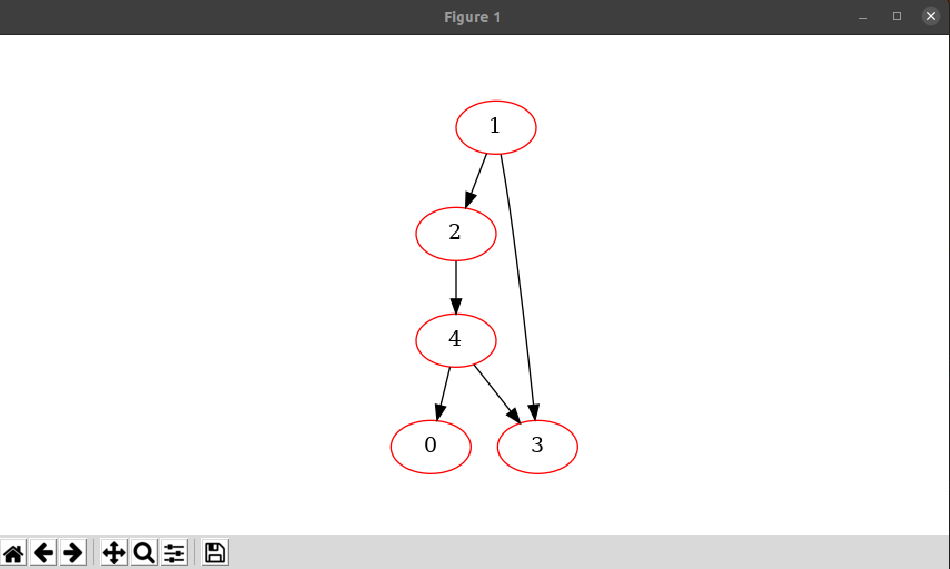
\includegraphics[width=\linewidth]{basic-graph.png}
  \caption{basic graph}
  \label{fig:basic graph}
\end{figure}
\bigskip
I will clarify that the node 4 is the one making a reference to the class. Now, we have a very interesting scenario. Our model has learned that our class variable only depends on the variable 1 and 2. Although at first glance it looks that our class only depends on the value of the nodes 1 and 2 remember that knowing information about nodes 0 and 3 can tell us hoe node 4 is conditioning them and thus give us information about our class
\bigskip
\begin{normalsize}
\textbf{3.2.2   Constraint graph} 
\end{normalsize}
This type of implementation will require us to provide the graph we saw above to the Bayesian network. In order to learn this graph we will run the exact algorithm for our variables without the classes then add the class to this graph and use this as the constraints.
\bigskip
at first glance this looks like it will take more time since we are running the algorithm twice but we have to keep in mind this scales super exponentially with each column we add so the first run will be quite faster. But what about the second run? Well this is were our constraint graph helps. This graph will tell the algorithm for witch for each variable witch ones has to take into account and in doing this we are reducing the amount of possibilities we check gets greatly reduced specially if we have a large amount of variables or set of values.
This first run trough our data will return us the following graph:
\bigskip
\begin{figure}[h!]
  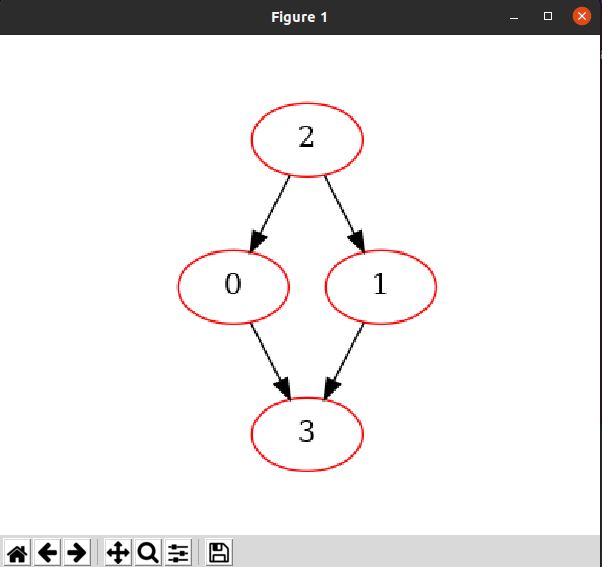
\includegraphics[width=\linewidth]{chi2-var.png}
  \caption{chi2 graph}
  \label{fig:basic graph}
\end{figure}
\bigskip
Note that even if we change from chi2 to f-regression we learn the same variables and the same graphs.
\bigskip
Now we will complete our constraint graph by adding a node, node number 4 and an edge from all the nodes to this one. We can observer how no matter where we start we will always end up in node 4 witch means that unlike the previous implementation all the information we get from the variables helps us predict the class
\bigskip
\begin{figure}[h!]
  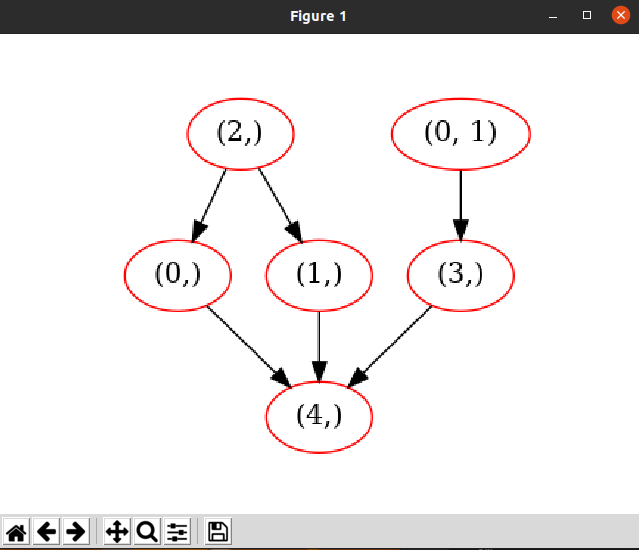
\includegraphics[width=\linewidth]{chi2-graph.png}
  \caption{Class constrain}
  \label{fig:basic graph}
\end{figure}
\bigskip
\bigskip
\bigskip
\bigskip
\bigskip
\bigskip
\bigskip
\bigskip
\bigskip
\bigskip
\bigskip
\bigskip
\bigskip
\bigskip
\bigskip
\bigskip
\bigskip
\bigskip
\bigskip
\bigskip
\bigskip
\bigskip
\bigskip
\bigskip
\bigskip
\bigskip
\bigskip
\bigskip
 We have our constraint graph completed. This graph will tell our Bayesian model witch nodes have an influence over witch. We run the exact A* algorithm again and we get our last graph. This graph if we do it correctly should look like the first one we got with the addition of the class node at the end feeding from all the information we have from the other variables.
\bigskip
\begin{figure}[h!]
  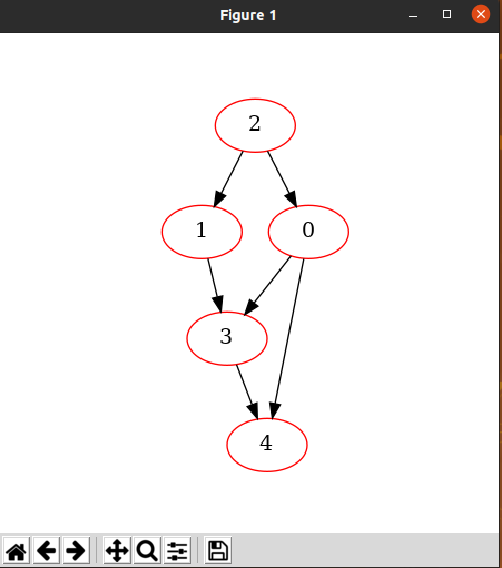
\includegraphics[width=\linewidth]{chi2-final-graph.png}
  \caption{chi2 final graph}
  \label{fig:basic graph}
\end{figure}
\bigskip
\bigskip
\bigskip
\bigskip
\bigskip
\bigskip
\bigskip
\bigskip
\bigskip
\bigskip
\bigskip
\bigskip
\bigskip
\bigskip
\bigskip
\bigskip
\bigskip
\bigskip
\bigskip
\bigskip
\bigskip
\bigskip
\bigskip
\bigskip
\bigskip
\bigskip
\bigskip
\bigskip
\bigskip
\bigskip
 
As i said earlier we have the first graph with our class node in the end.
\bigskip
\begin{normalsize}
\textbf{3.2.3   Other datasets}
\end{normalsize}
Up until now I have shown results that are from the breast cancer dataset. Nonetheless I also wanted to try this approach in a dataset less suited for Bayesian networks and by this I am talking about the digits dataset. Not only we have 64 variables now we have 9 classes and in order to get better results we will need to select a bigger proportion of variables to cover enough space.
\bigskip
I run the same process I described above but i chose 20 variables instead of for and Bayesian networks being super exponential in possible growth this made the time shoot up too. there we no changes needed in the implementation than loading the other dataset witch is a good sign if I want to use it for some other type of datasets.
\bigskip
Other than a way bigger graph and more time to calculate there where no other changes.
\subsection{Validation}
 
In order to validate this problem I made the choice to use 2 type of validation. First i checked the accuracy score since the problem is not very imbalanced it will give us a broad view of how the classifier is performing. The second measure I took is a confusion matrix, this will let us take a look at where the classifier is failing.
Basic implementation:
Accuracy score: 0.9084507042253521
\begin{table}[!h]
\centering
\begin{tabular}{lrrrr}
\toprule \hline
col\_0 &   0 &   1 & \\\hline
0     &  96 &   14 & \\\hline
1     &   12 &  162  \\\hline
\bottomrule \hline
\end{tabular}
\caption{Confusion matrix produced by the basic implementation classifier}
 \label{tab:BI}
\end{table}
This are actually very good results for a model that was implemented with no prior information of witch is the most important node so I am very happy with this results. Now lets take a look at our more complex model.
Graph with Constraints:
Accuracy score: 0.9049295774647887
\begin{table}[!h]
\centering
\begin{tabular}{lrrrr}
\toprule \hline
col\_0 &   0 &   1 & \\\hline
0     &  89 &   21 & \\\hline
1     &   6 &  162  \\\hline
\bottomrule \hline
\end{tabular}
\caption{Confusion matrix produced by the graph with constraints classifier}
 \label{tab:CG}
\end{table}
\bigskip
Lets take a look at how it performed in the digits dataset:
\bigskip
Basic implementation:
Accuracy score: 0.8062360801781737
The matrix was way to big and got deformed so i will use a picture to illustrate it for the digits problem
\begin{figure}[h!]
  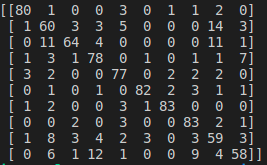
\includegraphics[scale = 1]{CFBI.png}
  \centering
  \caption{Confusion matrix for the basic implementation for digits}
  \label{fig:Confusion matrix for the basic implementation for digits}
\end{figure}
\bigskip
\bigskip

\bigskip
Lets take a look at the result from the implementation with the constraint graph.
\bigskip
Accuracy score: 0.46325167037861914
The matrix was way to big and got deformed so i will use a picture to illustrate it for the digits problem
\begin{figure}[h!]
  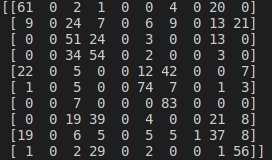
\includegraphics[scale = 1]{CFCG.png}
  \centering
  \caption{Confusion matrix for the basic implementation for digits}\hspace*{\fill}
  \label{fig:Confusion matrix for the constraint implementation for digits}
\end{figure}
\bigskip
Well these are some interesting result and i will gladly explain them and talk about them in the results section of these paper.
\section{Conditional Independence Tests}
I will talk now about the other form of using and building this bayesian networks. This is the approach I took:
\begin{enumerate} 
 \item Preprocessing of the dataset.
 
 \item Calculate the discrete distribution for each variable.
 
 \item Calculate the conditional probability table for the class.
 \item  Create a model using a graph.  
 
  \item  Select the appropriate evaluations methods and analyze the results . 
\end{enumerate} 
\subsection{Preprocessing}
In order to build this model we will apply a similar type of preprocessing to our dataset. Previously I talked about Trues and Falses, this is in fact an interpretation for the score based model we actually had '1.0' and '0.0' witch are in effect trues and falses, this will not suffice for this model. I will strictly substitute the values for the True and False values of python. This is in order to have a direct correlation between the values on our dataset, the values in all of our possible combinations and the values for our states. the rest of the preprocessing is identical as the one I presented before.
\subsection{Discrete distributions of our features}
In order to build our model we need to now how our features distribute their values, In order words what are the chances a variables takes a value in a vacuum. Since we have 2 values per feature we will count how many times a it takes the value True and infer the chances of taking the values false as 1 - P(True). Once this is done for each of our features we will be done with their distributions witch we will use in order to build our new model.
\subsection{Conditional probability table}
This part is a bit trickier but it will show case why this networks grow in cost this much and we for this showcase I decided to stick with simple terms like "True/False" and a modest amount of features.
\bigskip
First we need to compute all the possible combinations of values that our features can take. In our case  we have 2 values and 4 features: $2^{4}$ . So our model scales in combinations like $m^{n}$. Where 'm' is the number of our features take and 'n' the number of features we have.
\bigskip
First lets get all the combinations with repetition of size 4 for our Trues and Falses. Now in order to get the complete set of this we will calculate all the possible permutations of each of the possible combinations.
After we are done with this we should have a matrix of size 16x4 with every single possible value we can encounter in the dataset. Just to make the point if we had one more value and one more feature instead of 16 we would have 243 posible set of values.
\bigskip
Now for each set of values we need to search our dataset searching for all the instances we have for each. Once this is done we will count how many times we have a the class "True" and we will infer the false value. For each set of values we will append two rows to our conditional probability table one with the class "True" and the possibility of getting that class and one for the class "False" and the possibility for this class.
\bigskip
With this we have completed our conditional probability table witch will have two times the amount of rows than our previous value table and two more columns.
We will create our Bayesian network with this table and the discrete distributions of the features previously defined.
\subsection{Building the graph}
This graph is simple to make, we will create a state for each variable and one for the class using the discrete distributions and our table. then we will add an edge from our features to the class.
\bigskip
It should look  like this:
\begin{figure}[h!]
  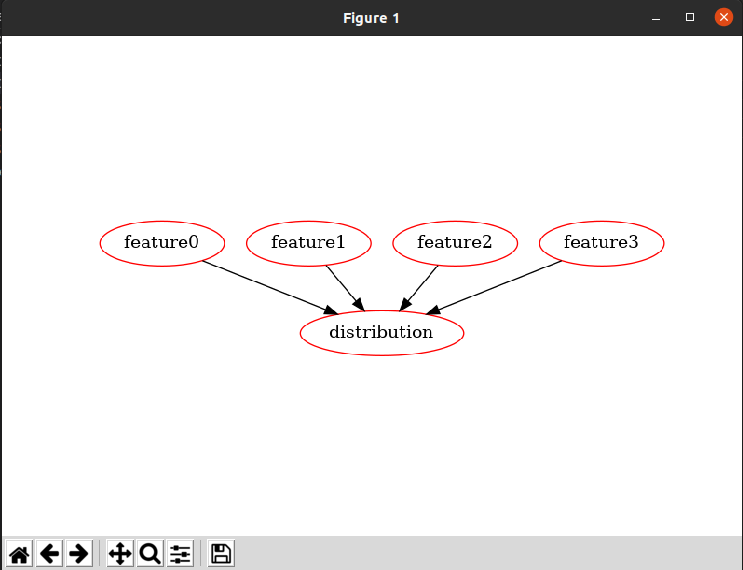
\includegraphics[scale = 0.7]{CI.png}
  \caption{Confusion matrix for the basic implementation for digits}\hspace*{\fill}
  \label{fig:Confusion matrix for the constraint implementation for digits}
\end{figure}
\subsection{Validation}
For validation we will follow the exact same steps and metrics as we did in the previous model.
Accuracy score: 0.8943661971830986
\begin{table}[!h]
\centering
\begin{tabular}{lrrrr}
\toprule \hline
col\_0 &   0 &   1 & \\\hline
0     &  107 &   3 & \\\hline
1     &   27 &  147  \\\hline
\bottomrule \hline
\end{tabular}
\caption{Confusion matrix produced by the graph with constraints classifier}
 \label{tab:CG}
\end{table}
\bigskip
This are results I am very happy about since we are getting almost all malign tumors with no error wich is the most important thing for this type of problem
\section{Implementation}
 All the project steps were implemented in Python. I used the datasets available in sklearn as well as some of their preprocessing tools. Most of the work is based on is the breast cancer dataset but I tried the same implementation using the digits dataset to see if i could get similar results with another problem. I used pomegranate in order to used they Bayesian networks library. To visualize the graphs we built I used networks since it works directly with pomegranate. Every test case and variation can be found in the folder by the name of code, this includes python notebooks and python files with the implementation.
\section{Results}
Looking at the results overall I can say they are pretty good with confidence, specifically happy with the Conditional independence model. Getting a bit more in depth with the score based network I would like to say that this gives us a better representations of how our data influences itself but it is also very costly without a constraint graph. Nonetheless we got very clear and more than adequate results in the 3 Bayesian networks tested in this paper.
\section{Conclusions}
Reaching the end I will give my final thoughts on the matter. First for the score based system. This is a very powerful way to build our network it will grind away until every single possible graph has been check and it will give us the one with the best results. Because of this, it is a very costly way of building networks. This is were constraint graph come to play, more over when we have even more features and a bigger set of values. Adding a constraint graph is not free it comes at a cost, if you don't know very precisely what the decencies are then you can make the mistake of giving the model false information and increasing the variance and the rate of mistakes. So be very careful how and when you use this.
\bigskip
On the Conditional independence test system. This is also a very costly system but instead of building all the possible graph what it does is it gets all the possible values you can encounter in your dataset, this is also a very thorough method and it has shown how well it performs in our test. If I had too chose one of these, I would have to chose this one. Even though it has a bit less accuracy it succeeds in the most important task while maintaining near 90\% accuracy, reducing the error of malign cancer detection.
\bigskip
As parting thoughts Ill tell you that the way you set up your data will play a crucial part on how your networks performs, changing the number of values features can take or witch value u use for them even the amount of features you take can radically change the outcome of your net, so think it through.
\section{Conclusions}
\begin{enumerate} 

\item Pomegranate: https://pomegranate.readthedocs.io/en/latest/

\item Pomegranate examples: https://github.com/jmschrei/pomegranate/tree/master/examples
 
\item A* Lasso : "https://www.cs.cmu.edu/~sssykim/papers/nips2013\_final.pdf"
 
\item Sklearn: https://scikit-learn.org/stable/index.html
 
\item Score based structure learning: https://ermongroup.github.io/cs228-notes/learning/structure/




\end{enumerate} 
\end{document}
